\documentclass[a4paper, 12pt]{report}

\usepackage[italian]{babel}
\usepackage{graphicx}
\usepackage{float}
\usepackage{tabularx}
\usepackage{ltablex}
\usepackage[font=small,format=plain,labelfont=bf,up,textfont=normal,up,justification=justified,singlelinecheck=false,skip=0.01\linewidth]{caption}
\usepackage{enumitem}
\renewcommand{\familydefault}{\sfdefault}

\title{Assignment 1 - Programmazione di reti\newline Anno accademico 2018-2019}
\date{\today}

\author{Matteo Castellucci - 0000825436\\Elena Rughi - 0000832797\\Yuqi Sun - 0000826197\newline}

\begin{document}

\maketitle

\tableofcontents

\chapter{Task Uno}

Per lo svolgimento del \textit{task} qui di seguito abbiamo fatto riferimento al \textit{file} ``task1.pcapng".

\section{Fase Zero}

Si sceglie l’interfaccia di connessione adoperata dal computer per accedere a Internet, sulla quale si effettua la cattura di pacchetti.

\begin{figure}[H]
	\centering
	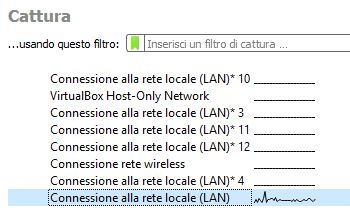
\includegraphics[width=\linewidth]{images/image1_1.png}
	\caption{Scelta dell'interfaccia su cui catturare i pacchetti}
\end{figure}

Avviata la cattura, si imposta il filtro ``tcp.port == 21" per filtrare i pacchetti che vengono scambiati durante la connessione FTP con il \textit{server ftp.ubuntu.com}, in quanto i 
\textit{server} FTP sono in ascolto sulla \textit{well-known port} 21. Una volta stabilita la connessione, si conosce l’indirizzo IP del \textit{server} e si può usare quest’ultimo per
filtrare i prossimi pacchetti, indipendentemente dalle porte coinvolte, tramite il filtro ``ip.addr == $<$server-IP-address$>$".
 
\section{Fase Uno}

Dal terminale, l'utente, utilizzando il \textit{client}, esegue il
comando ``ftp ftp.ubuntu.com" per iniziare la connessione; su Wireshark, si nota che il \textit{client}, da una propria porta impostata autonomamente, invia la richiesta di connessione alla porta
21 del server specificato. Una volta stabilita la connessione - la cosiddetta \textit{command connection} - sulla porta 21, il \textit{server} richiede al \textit{client} di inserire \textit{username}
e \textit{password}. Dopo che l'utente li ha forniti, il \textit{login} è completato. Anche questo scambio di pacchetti avviene sulla porta 21 del \textit{server}.

\begin{figure}[H]
	\centering
	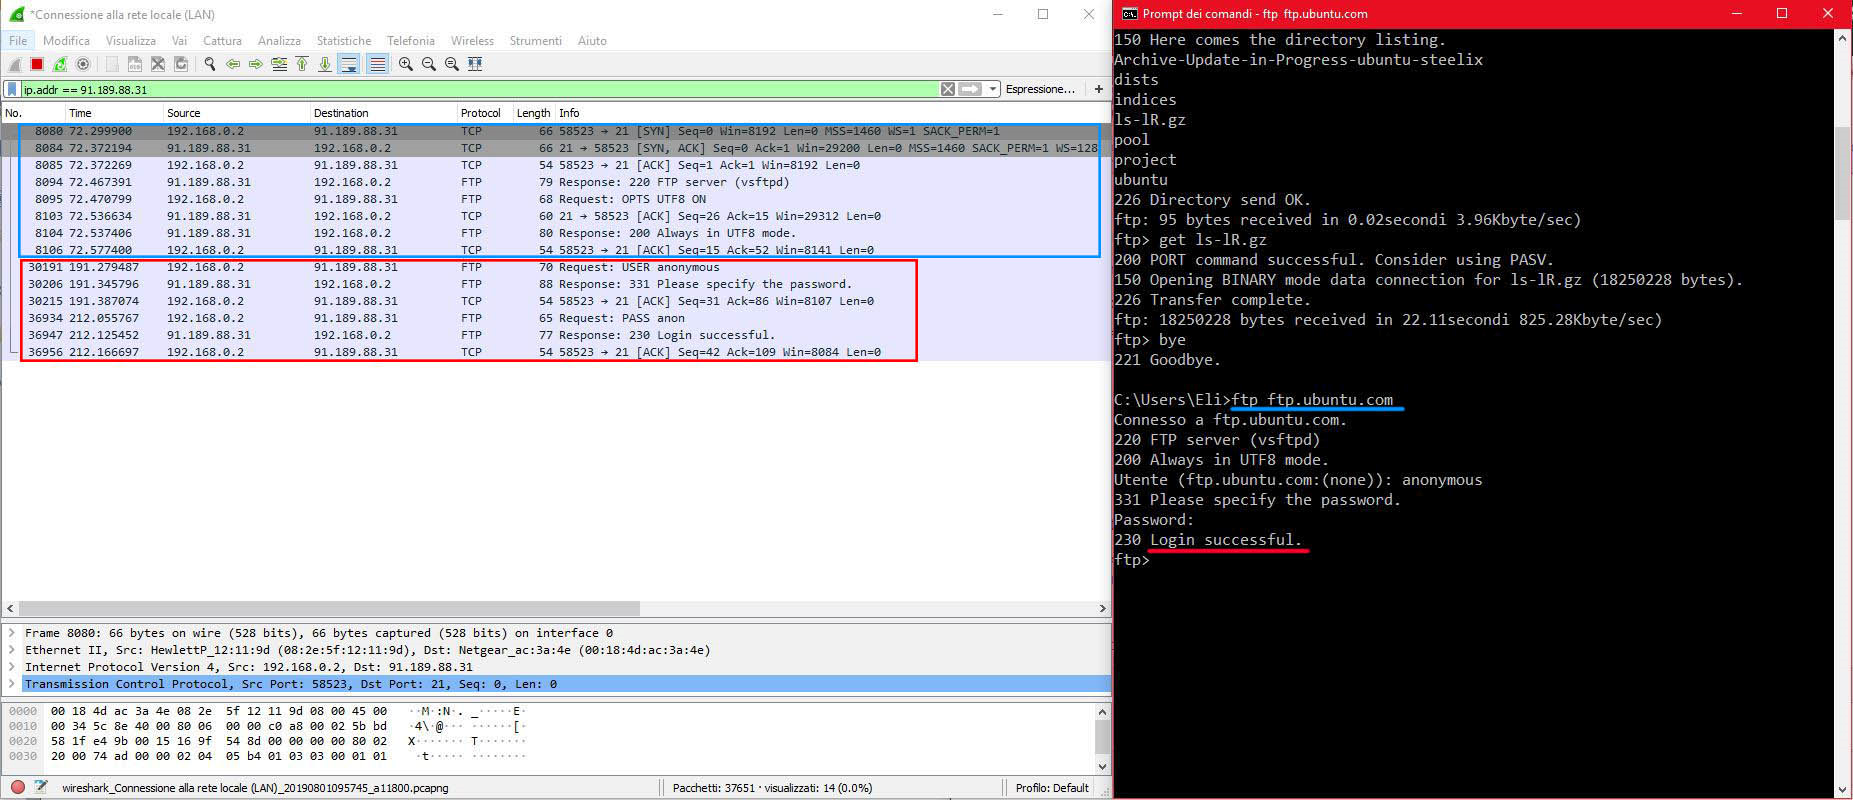
\includegraphics[width=\linewidth]{images/image1_2.png}
	\caption{Esecuzione della fase uno}
\end{figure}

\section{Fase Due}

La sequenza di comandi inviata dal client al server è stata la seguente:
\begin{itemize}
    \item ?: vengono visualizzati i comandi riconosciuti dal server ftp.ubuntu.com; in questo caso, non avviene alcuno scambio di pacchetti tra client e server.
    \item ls: si visualizza il contenuto della cartella corrente, che è costituito solamente dalla cartella ``ubuntu". Il client effettua una \textit{request} per stabilire una nuova connessione - detta 
    \textit{data connection} -, per la quale sia client che server riservano nuove porte, diverse dalle precedenti. Una volta inviati i pacchetti che contengono i dati, il server decide di effettuare
    la chiusura della connessione \textit{TCP} e stessa cosa decide di fare in seguito il \textit{client}.

    \begin{figure}[H]
        \centering
        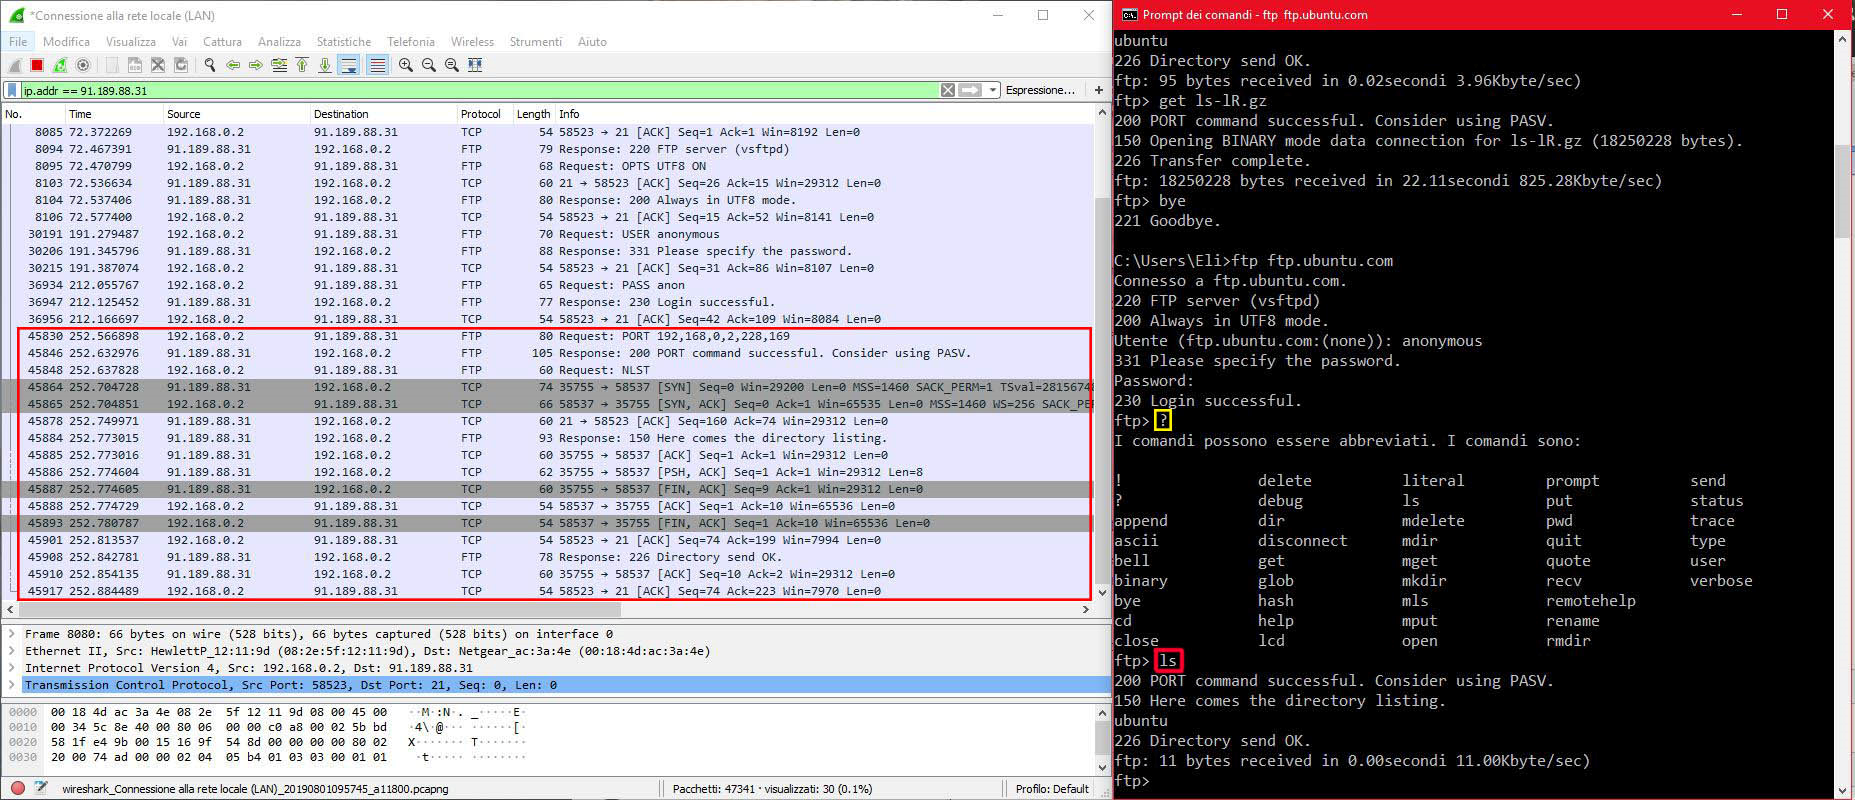
\includegraphics[width=\linewidth]{images/image1_3.png}
        \caption{Esecuzione del comando ``ls"}
    \end{figure}

    \item cd ubuntu: con questo comando si entra nella \textit{directory} specificata dopo il nome del comando stesso, \textit{directory} individuata tramite il precedente comando ls; questo comando viene eseguito tramite
    uno scambio di pacchetti che avviene esclusivamente sulla \textit{command connection} stabilita precedentemente. Nulla viene invece scambiato sulla \textit{data connection} per questo comando.
    \item ls: analogamente a prima, il \textit{client} stabilisce una nuova \textit{data connection}, che viene chiusa al termine dell’invio dei dati richiesti.
    
    \begin{figure}[H]
        \centering
        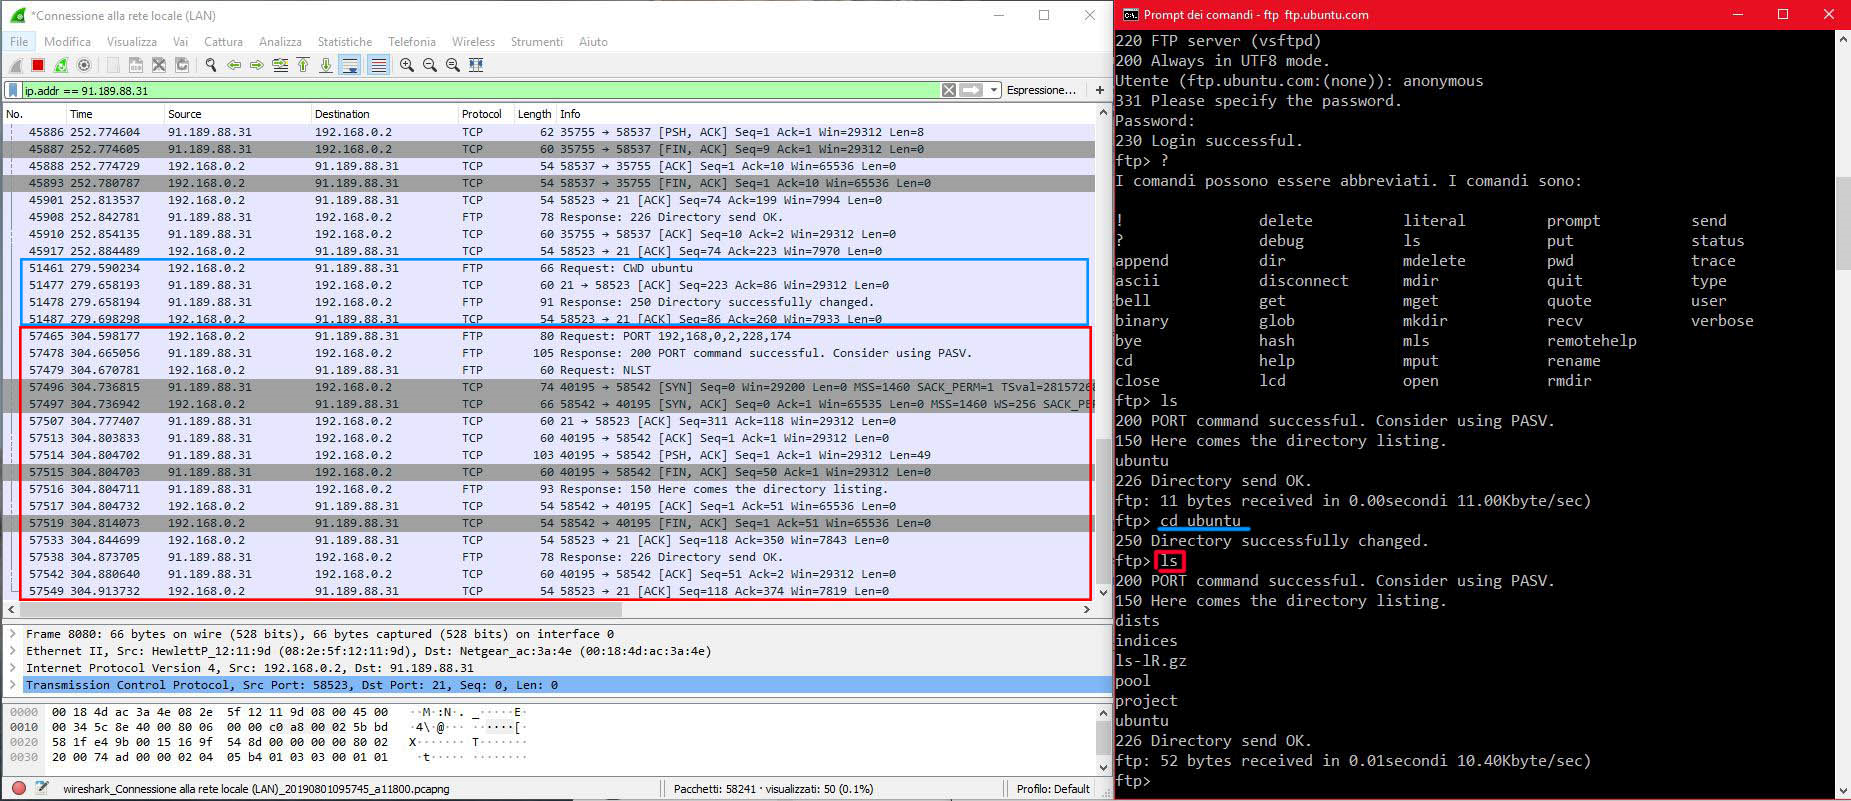
\includegraphics[width=\linewidth]{images/image1_4.png}
        \caption{Esecuzione del comando ``cd ubuntu" e del secondo comando ``ls"}
    \end{figure}

    \item get ls-lR.gz: il \textit{client} richiede al \textit{server} il \textit{file} ``ls-lR.gz"; viene stabilita una nuova \textit{data connection}, con nuove porte, poi il server inizia la trasmissione
    del \textit{file} attraverso questa connessione, similmente a quanto accadeva con il comando ``ls". Terminata la trasmissione del \textit{file}, il \textit{server} chiude la \textit{data connection} e in seguito anche il \textit{client}.

    \begin{figure}[H]
        \centering
        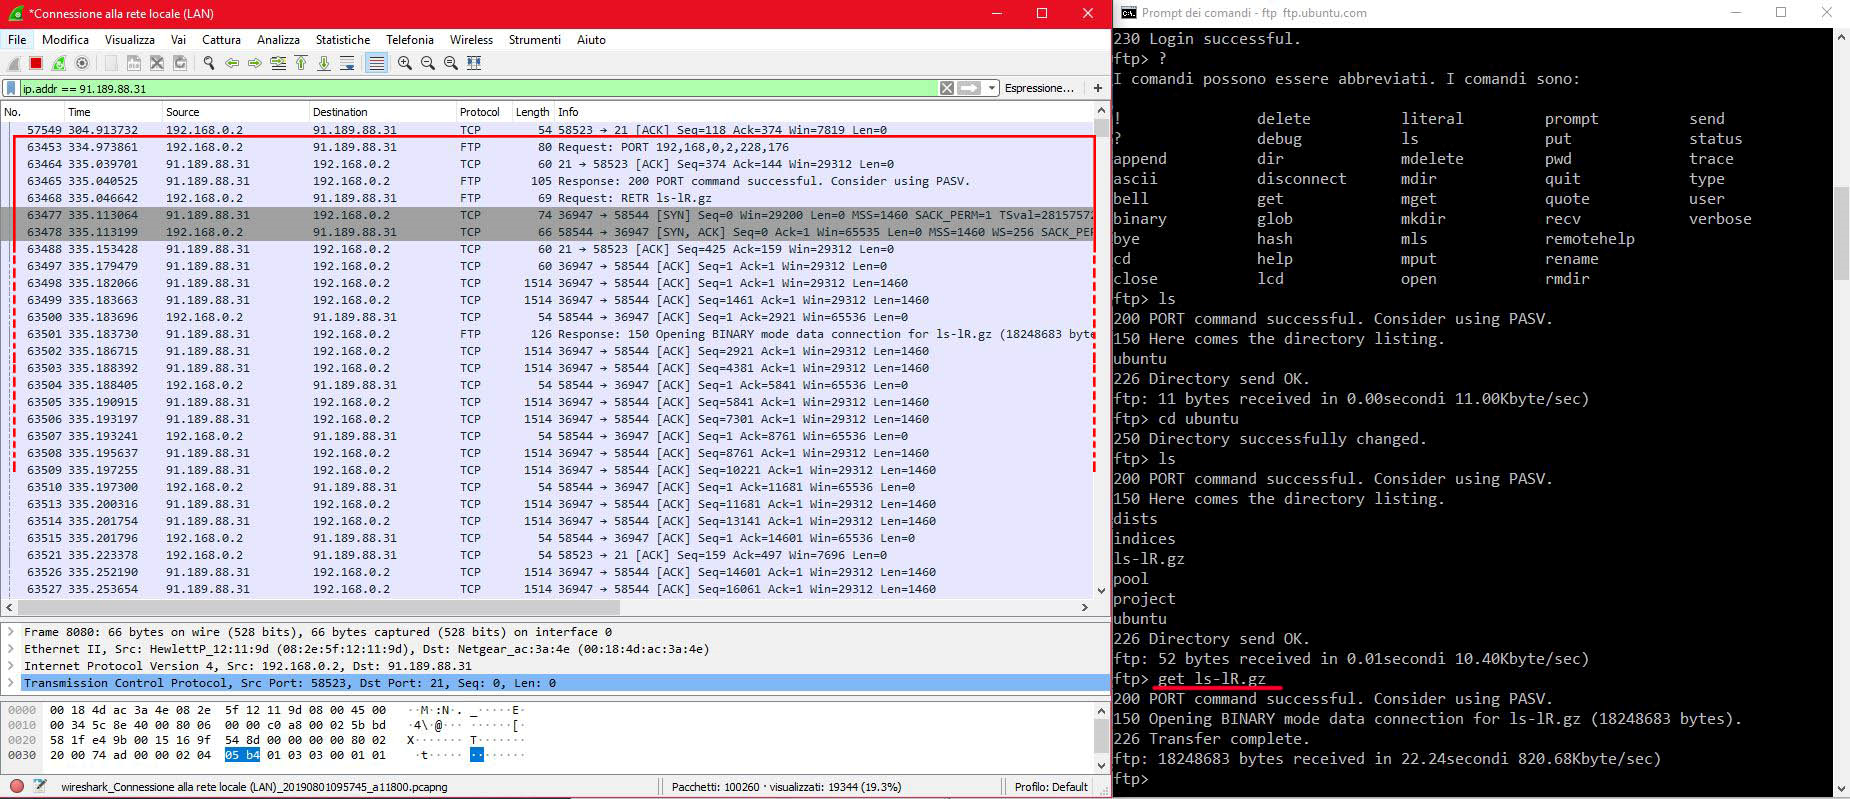
\includegraphics[width=\linewidth]{images/image1_5.png}
        \caption{Esecuzione del comando ``get ls-lR.gz"}
    \end{figure}

    \item bye: il \textit{client} segnala al \textit{server} che desidera terminare la connessione sulla \textit{command connection}, l’unica correntemente aperta.
    
    \begin{figure}[H]
        \centering
        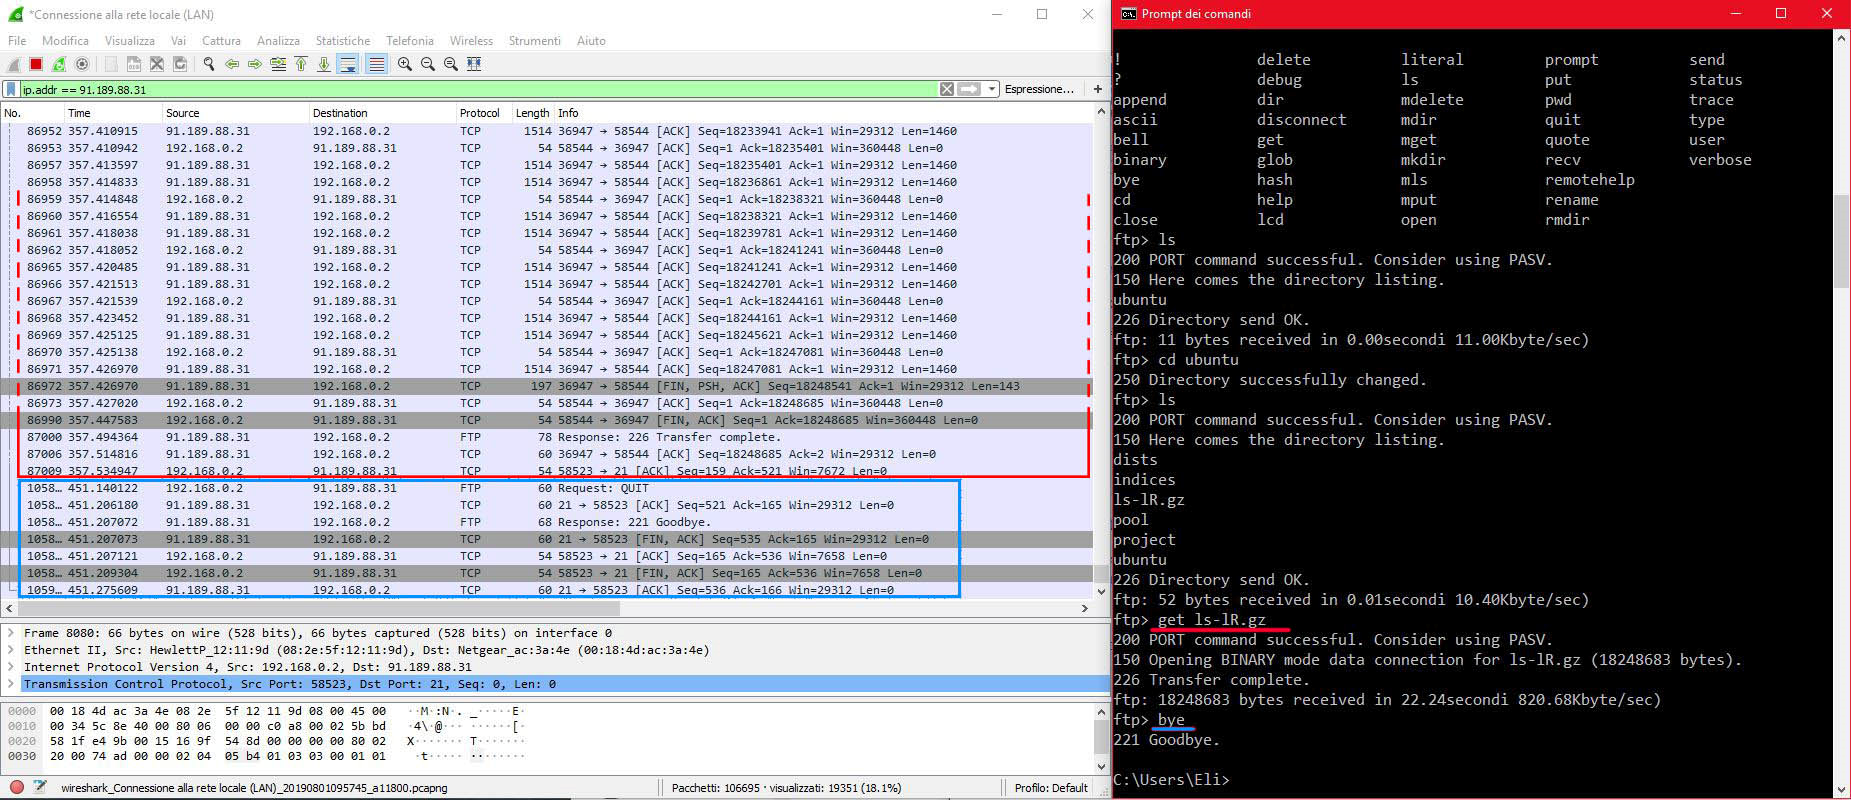
\includegraphics[width=\linewidth]{images/image1_6.png}
        \caption{Esecuzione del comando ``bye"}
    \end{figure}
\end{itemize}

\chapter{Task Due}

Per il \textit{task} due abbiamo fatto riferimento al file ``task2.pcapng" per rispondere alle domande. Nell'analisi dei messaggi sono stati ignorati i pacchetti inerenti al \textit{three-way handshake}
di TCP, i pacchetti di ``FIN" nonchè i pacchetti di ``ACK" perchè considerati non significativi per l'analisi dello scambio di messaggi del protocollo FTP. Infatti, questi pacchetti, essendo propri di TCP,
sono presenti in qualsiasi scambio di messaggi tra protocolli applicativi basati su TCP e non sono inerenti allo specifico protocollo FTP.

\section{Fase Zero}

\begin{enumerate}
    \item[\textbf{1.}] Il filtro migliore per visualizzare il traffico FTP è ``tcp.port == 21". Questo perchè permette di visualizzare
    solamente i dati che vengono scambiati attraverso la porta 21 del server, che sappiamo essere la \textit{well-known port}
    associata al protocollo FTP. Per poter visualizzare tutto il traffico che viene scambiato tra \textit{client} e \textit{server} durante
    la sessione però questo filtro non basta, ma occorre sfruttare l'indirizzo IP del server nel filtro ``ip.addr == $<$server-IP-address$>$",
    filtro che però può essere applicato solamente nelle fasi successive non sapendo noi a priori verso quale server - e perciò verso quale IP -
    stabiliremo una connessione. Quindi, in summa, il primo filtro indicato risulta essere il migliore.
\end{enumerate}

\section{Fase Uno}

\begin{enumerate}
    \item[\textbf{1.}] L'indirizzo IP del \textit{server} FTP è 91.189.88.31.
    \item[\textbf{2.}] La porta usata dal \textit{client} per iniziare la connessione FTP è la 53494.
    \item[\textbf{3.}] I messaggi FTP individuati in questa fase sono: \newpage
        \begin{tabularx}{\linewidth}{>{\hsize=0.25\hsize}X|X|>{\hsize=0.6\hsize}X|>{\hsize=0.475\hsize}X|>{\hsize=0.35\hsize}X|>{\hsize=0.375\hsize}X}
            \hline
            \textbf{N.} & \textbf{Messaggio} & \textbf{Tipo\newline messaggio} & \textbf{Tipo connessione} & \textbf{Porta\newline Client} & \textbf{Porta\newline Server}\\
            \hline
            \hline
            954 & 220 FTP server (vsftpd) & Response (Server $\rightarrow$ Client) & Comandi & 53494 & 21\\
            \hline
            955 & OPTS UTF8 ON & Request (Client $\rightarrow$ Server) & Comandi & 21 & 53494\\
            \hline
            961 & 200 Always in UTF8 mode. & Response (Server $\rightarrow$ Client) & Comandi & 53494 & 21\\
            \hline
            1513 & USER anonymous & Request (Client $\rightarrow$ Server) & Comandi & 21 & 53494\\
            \hline
            1518 & 331 Please specify the password. & Response (Server $\rightarrow$ Client) & Comandi & 53494 & 21\\
            \hline
            1671 & PASS & Request (Client $\rightarrow$ Server) & Comandi & 21 & 53494\\
            \hline
            1676 & 230 Login successful. & Response (Server $\rightarrow$ Client) & Comandi & 53494 & 21\\
            \hline
            \hline
            \caption{Messaggi scambiati durante la fase uno}
        \end{tabularx} 
    \item[\textbf{4.}] No, non sono presenti messaggi scambiati nella connessione dati in questa fase. Infatti, non sono state aperte altre connessioni
    oltre a quella correntemente in uso per i comandi, segno che non sono ancora stati scambiati dati tra \textit{client} e \textit{server}.
\end{enumerate}

\begin{figure}[H]
	\centering
	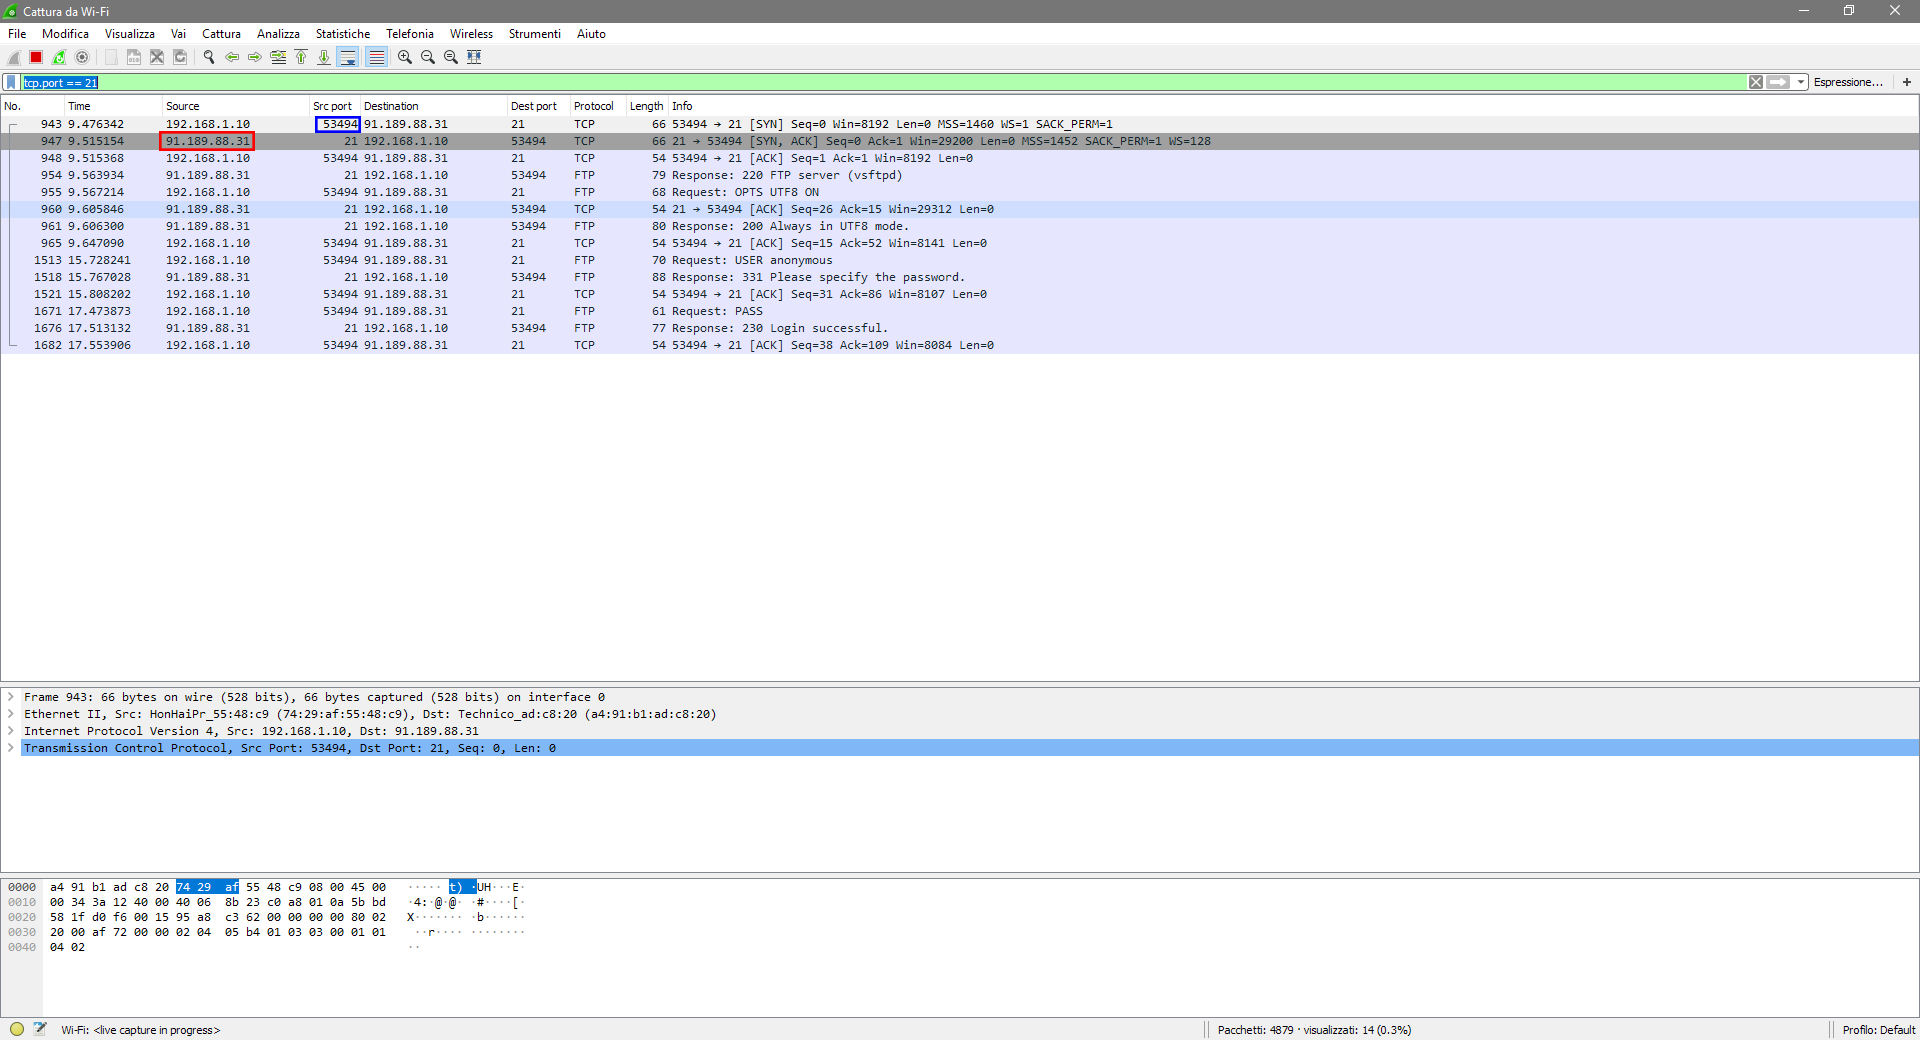
\includegraphics[width=\linewidth]{images/image2_1.png}
	\caption{Messaggi scambiati tra \textit{client} e \textit{server} nella fase uno}
\end{figure}

\begin{figure}[H]
	\centering
	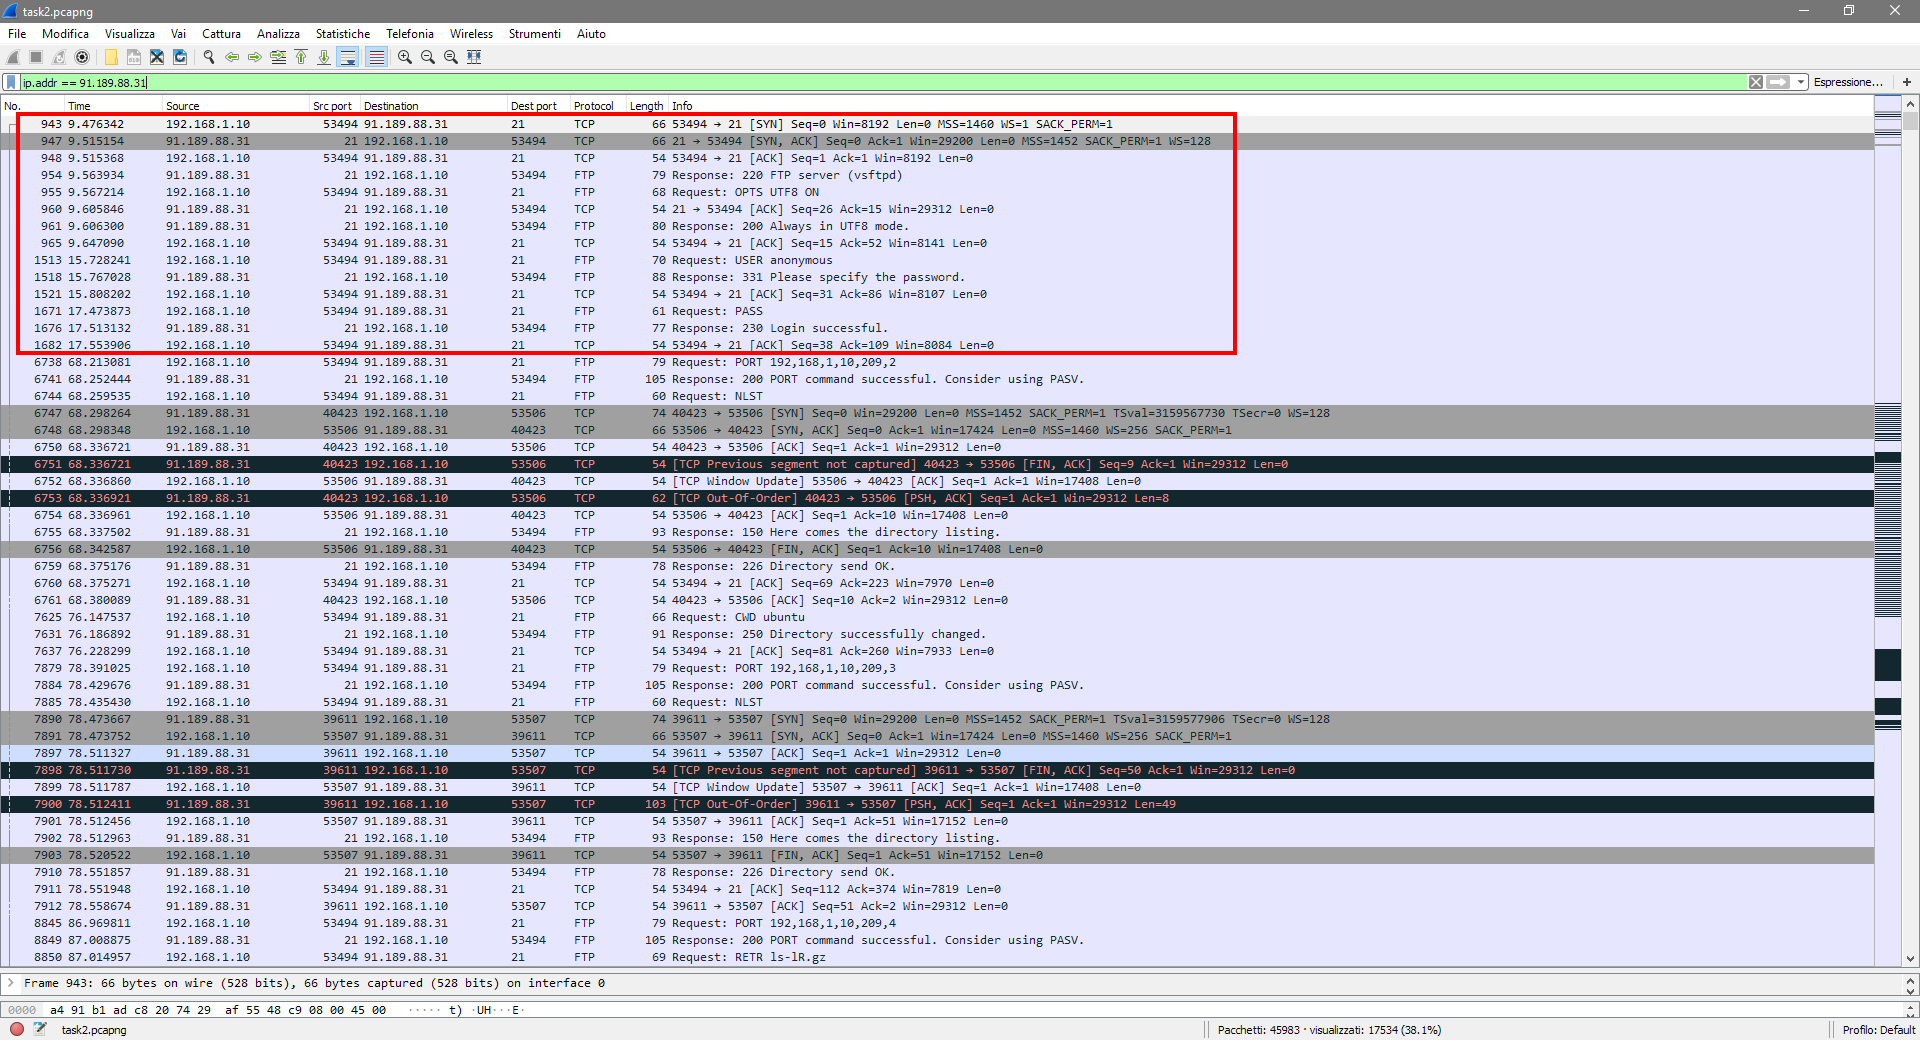
\includegraphics[width=\linewidth]{images/image2_1_1.png}
	\caption{Messaggi scambiati tra \textit{client} e \textit{server} nella fase uno visualizzati con il filtro ``ip.addr == $<$server-IP-address$>$"}
\end{figure}

\newpage

\section{Fase Due}

\begin{enumerate}
    \item[\textbf{1. 2.}] I messaggi \textit{FTP} individuati in questa fase sono:
        \begin{tabularx}{\linewidth}{>{\hsize=0.375\hsize}X|X|>{\hsize=0.35\hsize}X|>{\hsize=0.35\hsize}X}
            \hline
            \textbf{N.} & \textbf{Messaggio} & \textbf{Tipo messaggio} & \textbf{Tipo connessione} \\
            \hline
            \hline
            6738 & PORT 192,168,1,10,209,2 & Request & Comandi\\
            \hline
            6741 & 200 PORT command successful. Consider using PASV. & Response & Comandi\\
            \hline
            6744 & NLST & Request & Comandi\\
            \hline
            6747-6754, 6756, 6761 & \textit{Trasferimento dati inerente alla richiesta di directory listing} & & Dati\\
            \hline
            6755 & 150 Here comes the directory listing. & Response & Comandi\\
            \hline
            6759 & 226 Directory send OK. & Response & Comandi\\
            \hline
            7625 & CWD ubuntu & Request & Comandi\\
            \hline
            7631 & 250 Directory successfully changed. & Response & Comandi\\
            \hline
            7878 & PORT 192,168,1,10,209,3 & Request & Comandi\\
            \hline
            7884 & 200 PORT command successful. Consider using PASV. & Response & Comandi\\
            \hline
            7885 & NLST & Request & Comandi\\
            \hline
            7890-7901, 7903, 7912 & \textit{Trasferimento dati inerente alla richiesta di directory listing} & & Dati\\
            \hline
            7902 & 150 Here comes the directory listing & Response & Comandi\\
            \hline
            7910 & 226 Directory send OK & Response & Comandi\\
            \hline
            8845 & PORT 192,168,1,10,209,4 & Request & Comandi\\
            \hline
            8849 & 200 PORT command successful. Consider using PASV & Response & Comandi\\
            \hline
            8850 & RETR ls-lR.gz & Request & Comandi\\
            \hline
            8863 & 150 Opening BINARY mode data connection for ls-lR.gz (18250228 bytes) & Response & Comandi\\
            \hline
            8854, 8855, 8864-8880, 8884-26804, 26809 & \textit{Trasferimento dati inerente al file ls-lR.gz} & & Dati\\
            \hline
            26808 & 226 Transfer complete (trasferimento dati completo) & Response & Comandi\\
            \hline
            27596 & QUIT (richiesta di terminazione sessione) & Request & Comandi\\	    
            \hline
            \hline
            \caption{Messaggi scambiati durante la fase due}
        \end{tabularx}
    \item [\textbf{3.}] a) La \textit{data connection} è in tutti i casi aperta in modalità \textit{active} perchè è sempre il \textit{client} per primo a segnalare al \textit{server} tramite il comando ``PORT" a quale 
    \textit{socket} effettuare la connessione per lo scambio dei dati. È poi il \textit{server} in un secondo momento a decidere di aprire la connessione sulla base delle informazioni ricevute dal
    \textit{client}, comportamento di una \textit{data connection} aperta in modalità \textit{active}.
    \item [\textbf{3.}] b)
        \begin{tabularx}{\linewidth}{>{\hsize=0.5\hsize}X|X|>{\hsize=0.35\hsize}X|>{\hsize=0.275\hsize}X|>{\hsize=0.275\hsize}X}
            \hline
            \textbf{N.} & \textbf{Messaggio} & \textbf{Tipo connessione dati} & \textbf{Porta client} & \textbf{Porta server}\\
            \hline
            \hline
            6747-6754, 6756, 6761 & \textit{Trasferimento dati inerente alla richiesta di directory listing} & active & 53506 & 40423\\
            \hline
            7890-7901, 7903, 7912 & \textit{Trasferimento dati inerente alla richiesta di directory listing} & active & 53507 & 39611\\
            \hline
            8854, 8855, 8864-8880, 8884-26804, 26809 & \textit{Trasferimento dati inerente al file ls-lR.gz} & active & 53508 & 42077\\
            \hline
            \hline
            \caption{Messaggi scambiati durante la fase due}
        \end{tabularx}
    \item [\textbf{4.}]
        \begin{itemize}
            \item PORT 192,168,1,10,209,2: con il comando ``PORT" il \textit{client} dice al \textit{server} su quale indirizzo IP e quale porta sarà in ascolto per aprire la
            connessione dati
            \item PORT command successful. Consider using PASV: il \textit{server} comunica al \textit{client} di aver ricevuto correttamente e compreso il comando ``PORT".
	        Suggerisce di usare il comando ``PASV" per iniziare una connessione dati di tipo ``\textit{passive}"
            \item NLST: con ``NLST" si richiede la lista dei \textit{filename} nella \textit{directory} specificata (in questo caso quella corrente)
            \item \textit{Trasferimento dati inerente alla richiesta di directory listing}: messaggi per il trasferimento dei dati inerenti al \textit{directory listing}
            chiesto in precedenza
	        \item 150 Here comes the directory listing.: messaggio da parte del \textit{server} al \textit{client} che indica l'inizio del trasferimento dei dati inerenti al \textit{directory listing}
	        \item 226 Directory send OK.: messaggio da parte del \textit{server} al \textit{client} che indica l'avvenuto trasferimento con successo dei dati inerenti al \textit{directory listing}    
            \item CWD ubuntu: messaggio del \textit{client} per cambiare la directory corrente nella sottodirectory ``ubuntu"
            \item 250 Directory successfully changed.: messaggio del \textit{server} che indica il cambiamento della \textit{directory} effettuato con successo
            \item PORT 192,168,1,10,209,3: ha significato analogo a quello del comando ``PORT" precedente, ma il \textit{client} si mette in ascolto su una nuova porta, diversa
            dalla precedente
            \item PORT command successful. Consider using PASV: messaggio con significato analogo al precedente dello stesso tipo
            \item NLST: messaggio con significato analogo al precedente dello stesso tipo
            \item \textit{Trasferimento dati inerente alla richiesta di directory listing}: gruppo di messaggi con significato analogo ai precedenti dello stesso tipo
	        \item 150 Here comes the directory listing.: messaggio con significato analogo al precedente dello stesso tipo
	        \item 226 Directory send OK.: messaggio con significato analogo al precedente dello stesso tipo
            \item RETR ls-lR.gz: messaggio del \textit{client} per ottenere una copia del file ``ls-lR.gz"
            \item 150 Opening BINARY mode data connection for ls-lR.gz (18250228 bytes): messaggio del \textit{server} che specifica l'apertura di una \textit{data connection}
            in modalità ``BINARY" per il trasferimento del file richiesto, ``ls-lR.gz", che ha dimensioni pari a 18250228 bytes
            \item \textit{Trasferimento dati inerente al file ls-lR.gz}: gruppo di messaggi inviati sulla \textit{data connection} appena aperta che effettuano il
            trasferimento del file dal \textit{server} al \textit{client}
            \item 226 Transfer complete (trasferimento dati completo): messaggio del \textit{server} che indica il completamento del trasferimento del \textit{file} richiesto
            \item QUIT (richiesta di terminazione sessione): messaggio del \textit{client} per richiedere la chiusura della \textit{command connection} correntemente aperta
        \end{itemize}
\end{enumerate}

\begin{figure}[H]
	\centering
	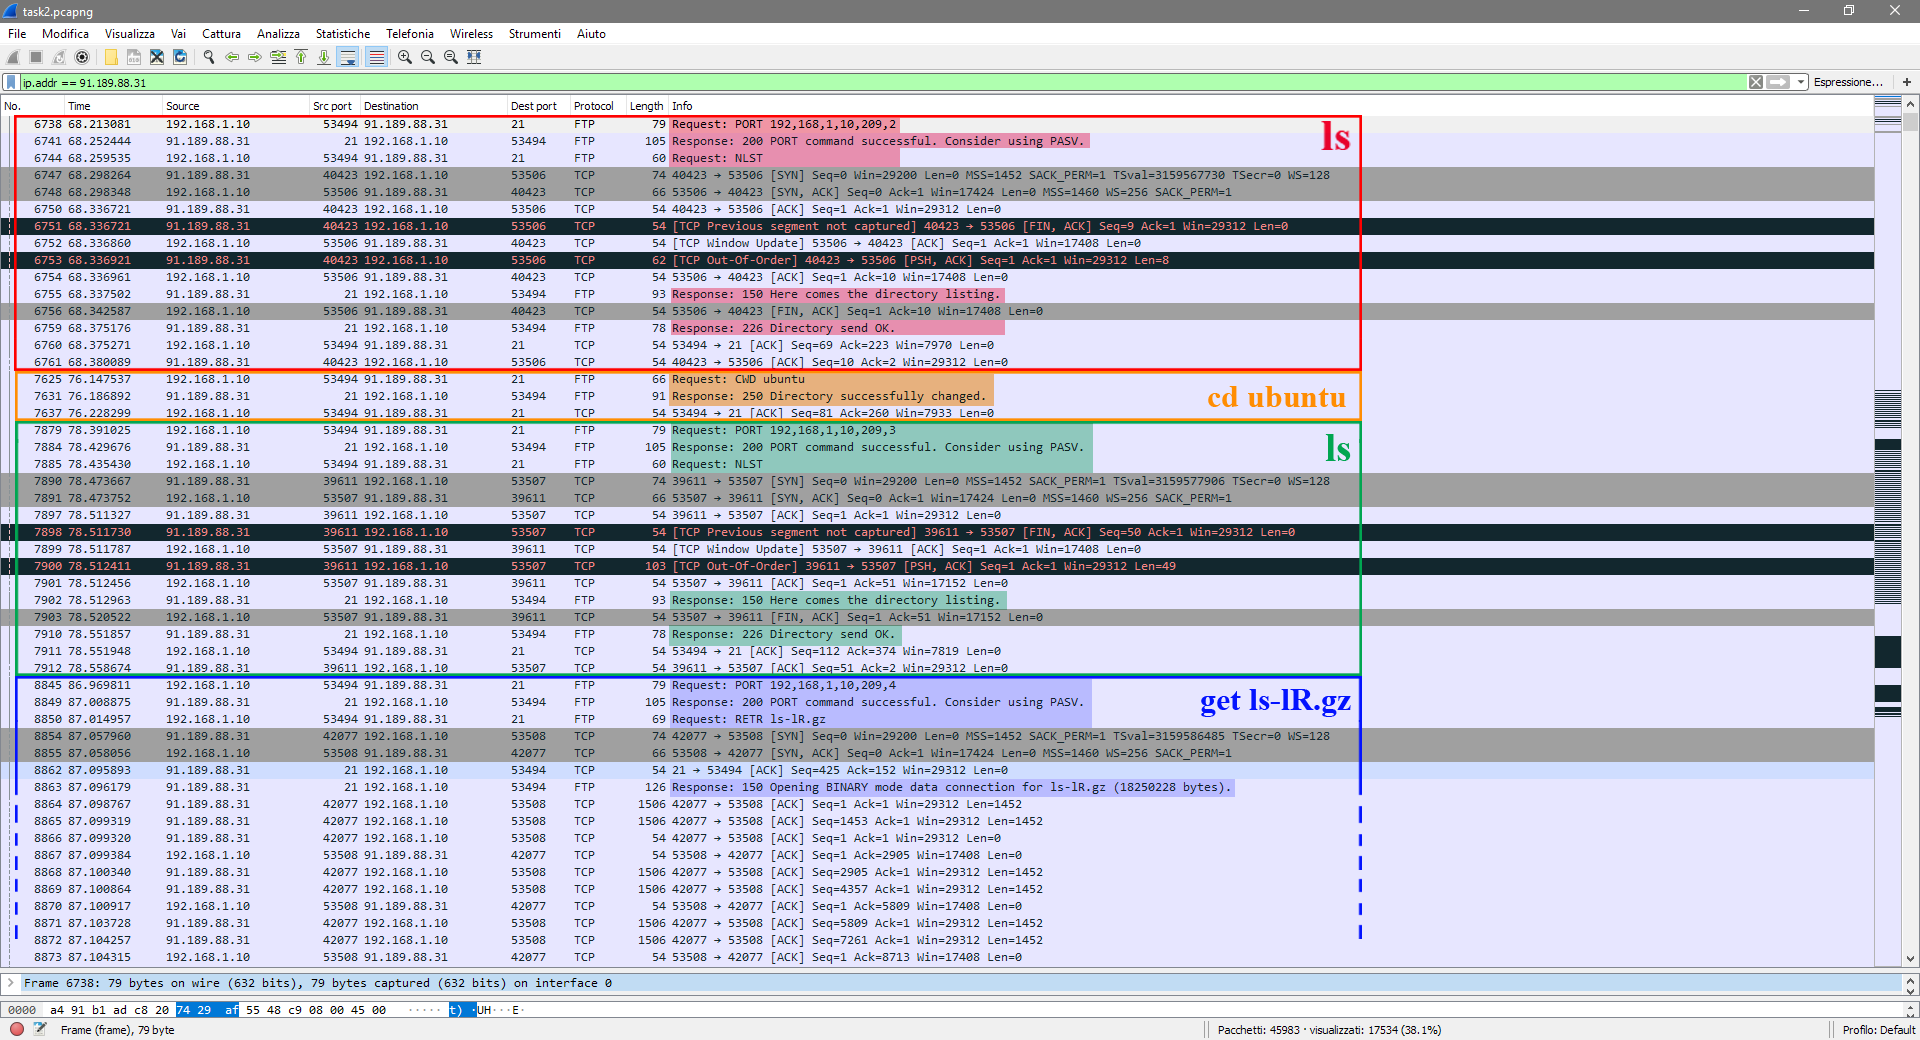
\includegraphics[width=\linewidth]{images/image2_2.png}
	\caption{Messaggi scambiati tra client e server durante la fase due}
\end{figure}

\begin{figure}[H]
	\centering
	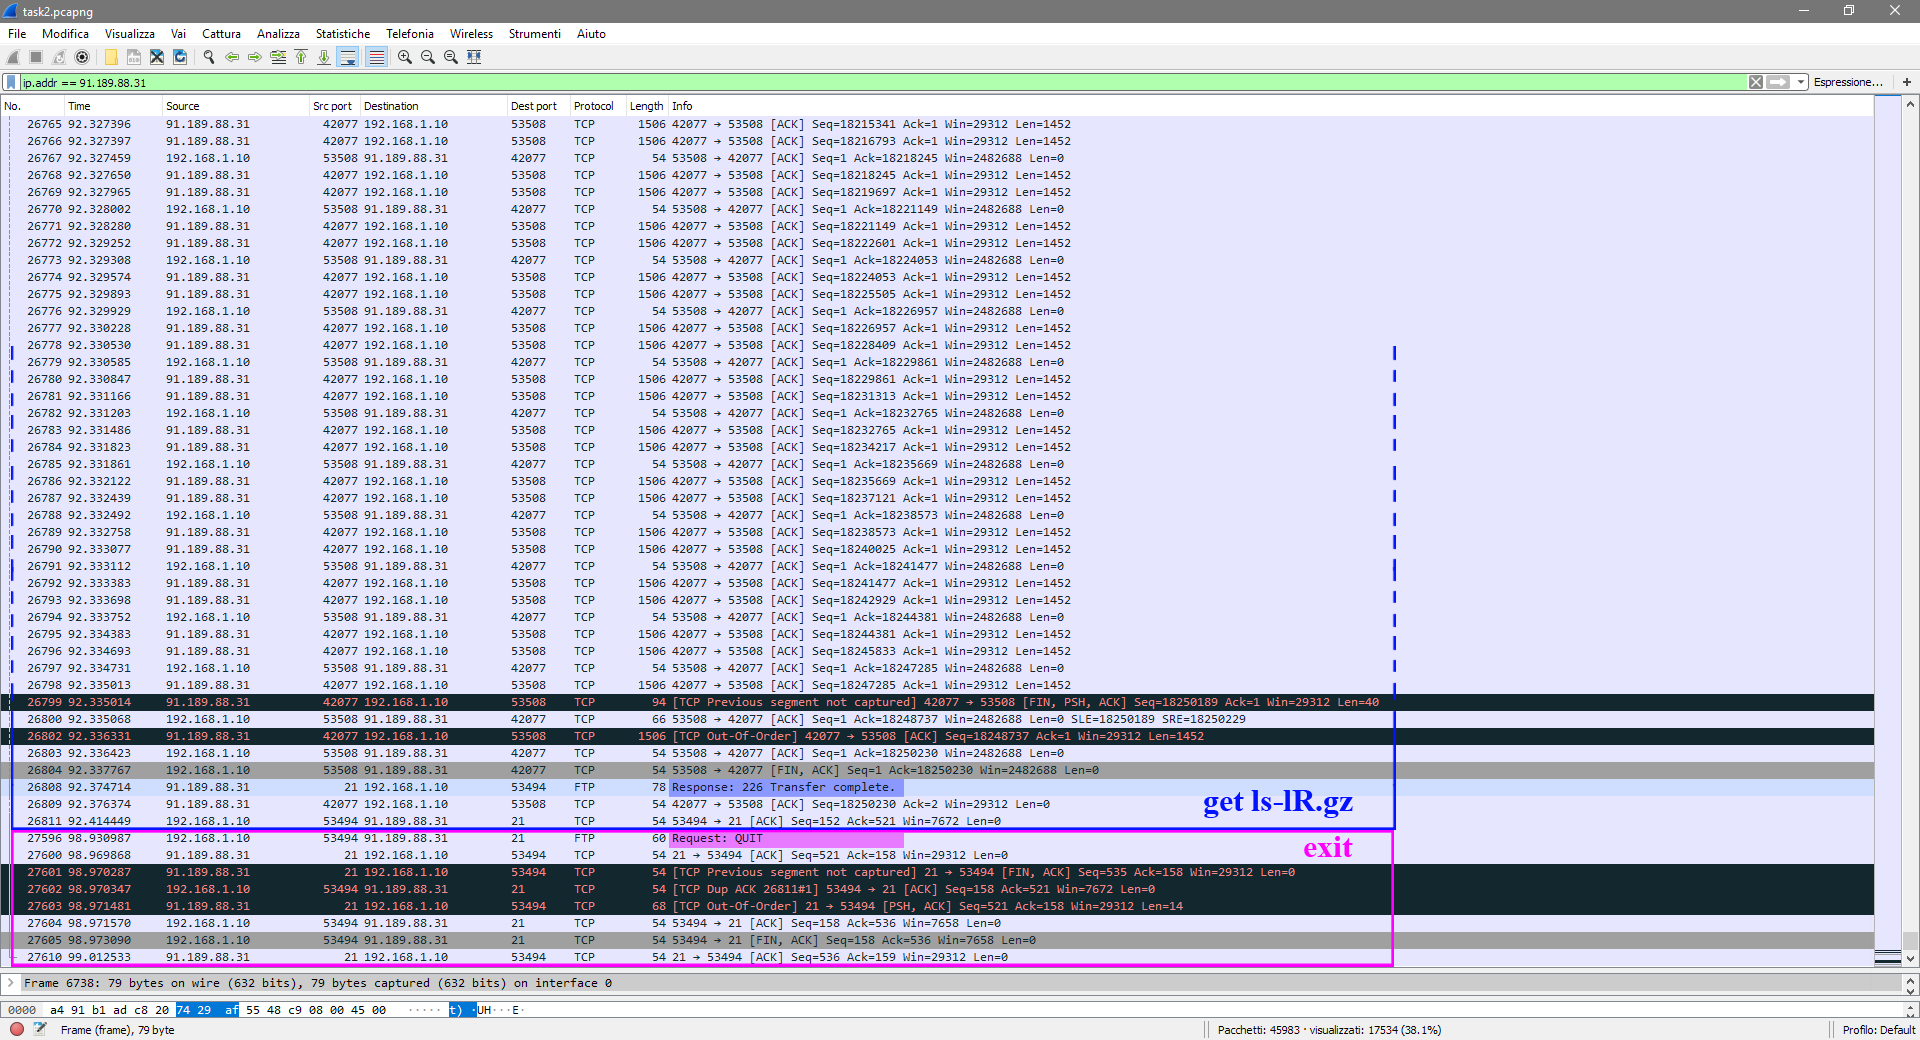
\includegraphics[width=\linewidth]{images/image2_3.png}
	\caption{Messaggi scambiati tra client e server durante la fase due}
\end{figure}

\end{document}
